% !TEX root = ../main.tex
\section{VeriNC}

\begin{frame}{VeriNC}
  \begin{center}
    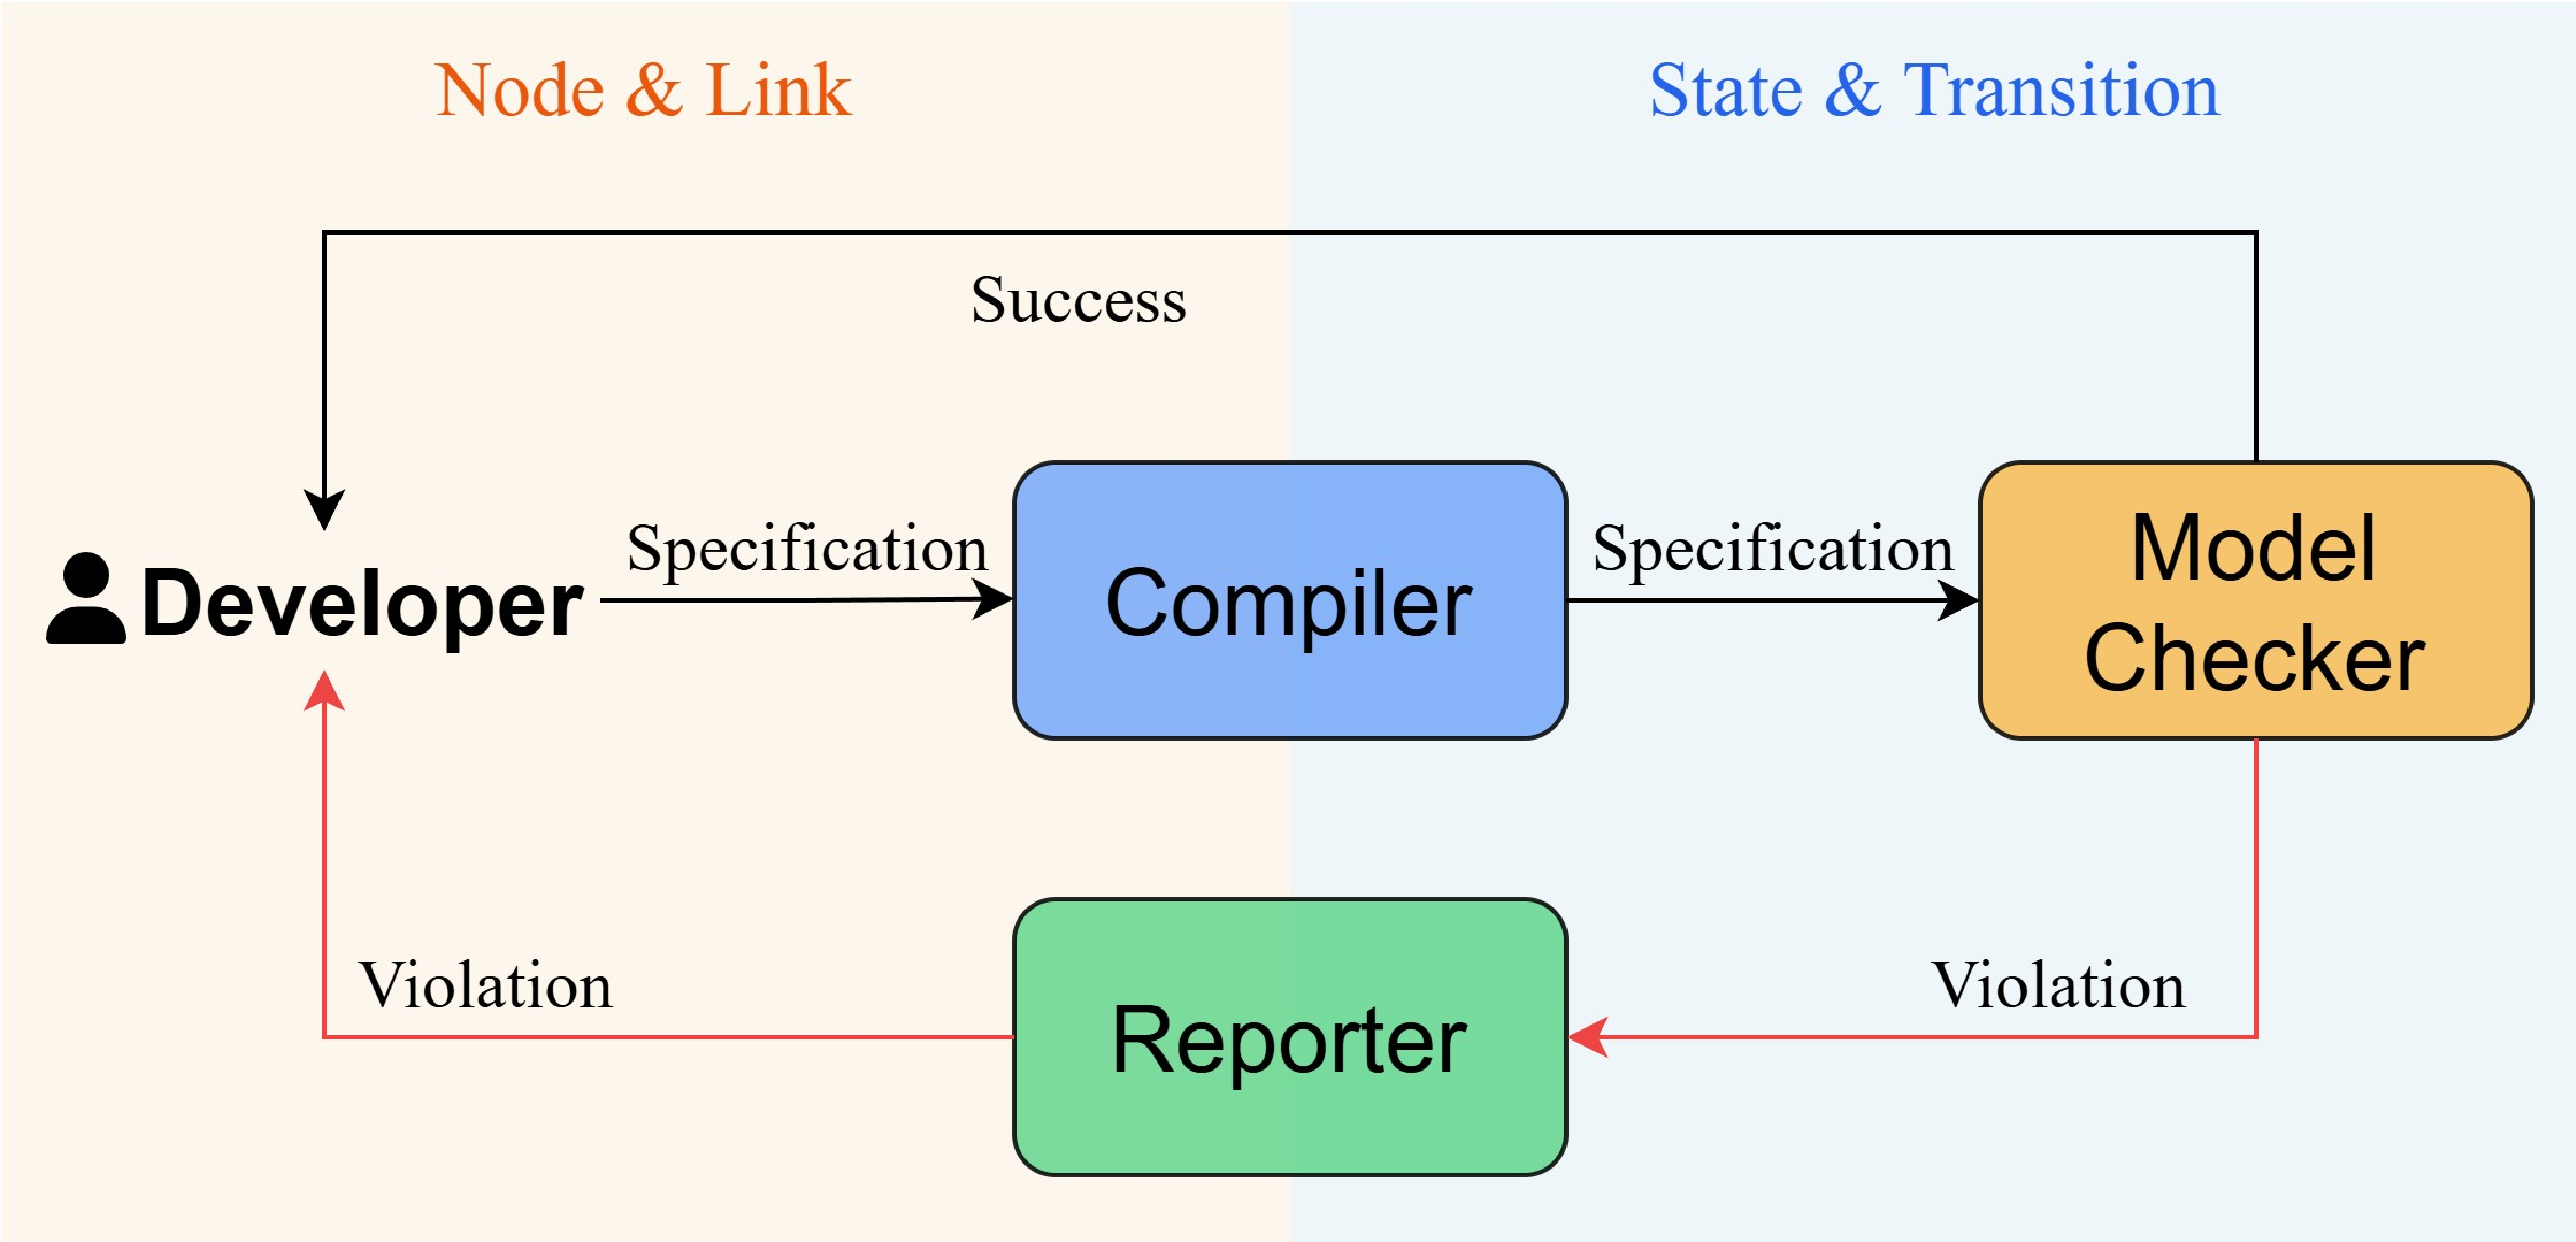
\includegraphics[width=0.70\textwidth]{figures/workflow.pdf}
  \end{center}
  \vspace{0.7em}
  \begin{center}
    \begin{minipage}{0.90\textwidth}
      \centering
      \alert{\textbf{VeriNC explores all possible execution traces ---
      exhaustively, within the bounds you set.}}
    \end{minipage}
  \end{center}
  \speechnote{7}
\end{frame}

\begin{frame}{The Abstraction You Work In}
  \vspace{0.5em}
  \begin{itemize}
    \item A \textbf{node} is a machine, running several \textbf{threads} ---
          application, receive, retransmission.\\
          {Threads run concurrently; every interleaving gets explored.}
    \vspace{0.7em}
    \item<2-> Nodes are joined by \textbf{links}. Three primitives:
          \texttt{Send}, \texttt{Receive}, \texttt{Multicast}.
    \vspace{0.7em}
    \item<3-> The network is \textbf{reliable}, \textbf{lossy}, or \textbf{out-of-order} ---
          set globally, or per link.
  \end{itemize}
  \vspace{1.0em}
  \visible<4->{%
    \begin{center}
      \begin{minipage}{0.92\textwidth}
        \centering
        % 手动断行：自己折的话 "itself." 会单独掉到第二行
        \alert{\textbf{Users specify protocol behavior\\
        without modeling the network itself.}}
      \end{minipage}
    \end{center}}
  \speechnote{8}
\end{frame}

\begin{frame}[fragile]{What You Actually Write}
  \vspace{0.2em}
  \begin{center}
    \begin{minipage}{0.88\textwidth}
\begin{lstlisting}[style=spec, basicstyle=\ttfamily\footnotesize]
configuration {
  MAX_LOSS = 1;  CLIENT_NUM = 3;  REQ_NUM = 5;  ...
}
topology {
  nodetype Client, Switch, Controller, Server;
  link c1, c2, c3 -- sw -- ctrl, s;  ...
}
protocol {
  var(Switch) cached = 0, valid = 0, value = null;  ...
  thread(Switch) SwitchRecv { ... }
}
\end{lstlisting}
    \end{minipage}
  \end{center}
  \vspace{0.4em}
  \begin{center}
    \alert{Protocol logic, not P4 --- the core logic, without implementation detail.}
  \end{center}
  \speechnote{9}
\end{frame}

\begin{frame}[fragile]{Saying What Correctness Means}
  \vspace{1.2em}
  \begin{itemize}
    \item An \textbf{assert statement} --- a first-order logic formula,
          checked where it sits
    \vspace{1.0em}
    \item A \textbf{property} block in LTL, checked after every transition\\[0.4em]
          \hspace*{1.2em}\texttt{[]} always \qquad \texttt{<>} eventually
    \vspace{1.0em}
    \item A \textbf{stateful check function}, for complex temporal properties
  \end{itemize}
    \speechnote{10}
\end{frame}
